\documentclass[10pt,letterpaper]{report}
\usepackage[utf8]{inputenc}
\usepackage{amsmath}
\usepackage{amsfonts}
\usepackage{amssymb}
\usepackage{graphicx}
\usepackage[usenames, dvipsnames]{color}
\usepackage{textcomp}
\usepackage{mathtools}
\usepackage[left=2cm,right=2cm,top=2cm,bottom=2cm]{geometry}
\author{Brandon Caudell}
\title{Combinatorics of Rubik's Cubes}
\DeclarePairedDelimiter\ceil{\lceil}{\rceil}
\DeclarePairedDelimiter\floor{\lfloor}{\rfloor}
\definecolor{darkgreen}{RGB}{0, 128, 0}
\begin{document}
\maketitle
\newpage 
\tableofcontents
\newpage 
\chapter{Introductory Information}
\section{Origins of the Rubik's Cube}
\section{Basic Terminology}
The standard 3x3 Rubik's Cube has six colors, one for each face.  The typical color scheme is white, yellow, red, orange, green, and blue.  The cube contains 26 external pieces, known as \textbf{cubies} or simply pieces.  These cubies come in 3 variants: \textbf{centers}, \textbf{edges}, and \textbf{corners}.  Center cubies contain only one colored sticker, edge pieces contain two stickers, and corner cubies contain three stickers.\\

Each of the cube's six faces can be independently rotated by multiples of 90\textdegree.  When held in a particular position, the six faces of the cube are generally regarded as front, back, left, right, up, and down.  These terms give rise to the standard move notation of F,B,L,R,U,D to denote clockwise rotations by 90\textdegree of each face.\\

These six moves are enough to scramble and solve the puzzle in any possible way, though it is convenient to define addition moves for clarity.  An apostrophe is used to denote a counter-clockwise move, so F' is a counter-clockwise rotation about the front face.  Adding a superscript 2 denotes performing a move twice, i.e. a 180\textdegree rotation, so $B^2$ is a 180\textdegree rotation of the back face.  This is regarded as a half-turn.  Note that by symmetry of the square faces, performing a clockwise move twice is equivalent to performing the counter-clockwise version twice, i.e. $L^2 \cong (L')^2$, so we just use the first notation.  Also note that repeating a clockwise-move (quarter-turn) three times is equivalent to a single counter-clockwise move, and vise versa.\\

Occasionally, it is useful to talk about \textbf{slice} moves.  These are moves obtained by rotating any of the three central "slices" of the cube.  In the standard 3x3 cube, these are denoted by lowercase variants of the same 6 letters, with apostrophes and exponents having the same meaning as before.  Note that if we talk about a slice relative to a particular face, that face still defines the direction of the rotation, but we actually rotate the cubies one layer "deeper" into the cube.  These slice moves are isomorphic at the cube level to performing two face turns on opposite faces, i.e. the slice move $r \cong R'L$ (rotating the right face counter-clockwise and the left face clockwise).  Although the two move sequences are isomorphic, they leave the cube as a whole oriented differently, hence why it is useful to define them even if they are rarely used in the 3x3 cube.  \\

We need to establish a convention in how to read these move sequences.  Since moves, in general, are not commutative, reading a sequence of moves such as $LFR$ from right-to-left or left-to-right changes the resulting cube.  While mathematically this sequence of moves is very similar to function composition, which is typically done right-to-left, it is easier for us to "read off" a move sequence left-to-right, so that is the convention that we will operate under.  In cases where a right-to-left order makes sense, we will formally declare that distinction. \\

Note that when applying face moves to a cube, the center cubies remain fixed.  The four edge and four corner pieces on a face will rotate around, but the centers always maintain the same orientation relative to each other.  This extends to slice moves as well (since slice moves can be attained by a composition of face turns), but note that in slice moves the centers may move on the cube as a whole.  Their relative orientations, however, always remain the same.  In the standard coloring, white is opposite yellow, red is opposite orange, blue is opposite green, and if white is held as the bottom face then blue is to the left of red.  Because of these fixed centers, when solving a cube, the solver always knows what color a face must end up.
\section{Larger Cubes}
Unsurprisingly, larger cubes present more options.  Not just in the number of permutations that can be obtained, but in the number of different cases one must handle when solving.  Thus, our notation and understanding must adapt to different cube sizes.  In this report, we denote the size of a cube as its \textbf{order}, i.e. an order-3 cube is the standard 3x3 one.  Note that larger cubes may have multiple center cubies, and they need not be at the centers of faces.  We still use this terminology, though. \\

For cubes of higher order, we gain additional move options.  Whereas on the standard cube, we only needed 6 moves to scramble and solve, we will need 3 more moves for each increase in order by 1.  A proof of this fact will be given later, but we will outline the notation here.  We still use capital letters to denote face moves, and these 6 moves will never change even as order increases.  As the size of the cube goes up, what will change is the number of distinct slice moves that can be performed.  For a cube of order $r$, there are $\floor{\frac{r}{2}}-1$ \textit{indecomposable} slice moves for each face.  By indecomposable, we mean moves not isomorphic to any other move sequences (so the slice moves in our 3x3 cube are decomposable and therefore less important).  For the standard cube, this gives that there are no indecomposable slice moves.  For the 4x4 cube (also known as the Rubik's Revenge), there is one slice move per face.\\

To denote which slice move we are talking about (as there may be many for large cubes), we use a subscript indexed from 1 to this $\floor{\frac{r}{2}}-1$.  In the case of the order-4 and 5 cubes, we may also use the lower-case letter variant as before, i.e. $r = R_1$.  Primes and powers still work as before.  While slightly clunky, this notation allows us to unambiguously denote which move is being performed. \\

One important consideration with larger cubes is the presence or absence of fixed centers.  As we showed, the 3x3 cube has center cubies that never change orientation.  This is true of all odd-order cubes, as the only moves that would move the centers at all can be decomposed into other moves that leave the centers untouched (possibly with a rotation of the cube as a whole in order to maintain directionality).  Even-order cubes, however, lose this nicety.  Since every move is unique and indecomposable, and there are multiple center cubies that will move independently of each other, it is up to the solver to ensure that the faces are actually reassembled in the correct relative orientations.  Not only must all colors be reassembled opposite their correct opposing color, but the relative orientations must be correct as well.  For instance, the white-red-blue corner piece is oriented such that the blue face should be left of red if the white face is pointed down.  If this orientation is not upheld, then the solve will not complete.
\chapter{Groups in the Rubik's Cube}
The first obvious question regarding the Rubik's Cube is ``How many possible scrambled states can the puzzle be in?''.  In order to answer this question, we need to understand the cube and its moves as an algebraic group.  We will start at a larger group and refine it down to our answer.
\section{The Sticker Group}
Given a cube of order $n$, it is easy to count the total number of stickers on it to be $6n^2$.  These stickers are partitioned into 6 different colors, one color per face on the solved cube.  Although clearly each sticker is ``locked'' to a cubie and thus the locations on the cube it can be moved to via legal moves are very limited, it is useful to think about what could happen if this constraint were removed. \\

If we were to take all the stickers off of the plastic cube body and rearrange them with no restrictions, then in how many ways could we do this?  If we assume each sticker is distinguishable (two red stickers can somehow be differentiated), then this sticker arrangement is just a permutation of $6n^2$ items.  We denote the algebraic group of these sticker rearrangements as the \textbf{Sticker Group of order n}.  The symbol we will use for this is $\mathcal{S}_n$.  This group is isomorphic to the symmetric group of order $6n^2$ for obvious reasons.  Thus, $\mathcal{S}_n \cong \mathfrak{S}_{6n^2}$. \\

Clearly, this is an extremely loose upper bound on the number of possible states of a valid Cube.  Let us go one level closer to the answer to our question.

\section{The (Re)assembly Group}
Permuting the stickers around is not really the group action we care about.  We would much rather consider actions on the cubies themselves, since those are the pieces being moved in legal rubiks moves.  Let us consider the group formed by arbitrarily taking the cube apart (leaving the stickers alone) and reassembling the cubies.  This group on a cube of order $n$ will be known as the \textbf{(Re)assembly group} of order $n$, denoted $\mathcal{R}_n$.  There will be a number of restrictions imposed on us by the physical nature of the cube, and we will account for these one at a time.

\subsection{Cubie Type Restrictions}

The reassembly group structure with the fewest restrictions will only respect the cubie types.  Corners must remain corners, etc.  Thus, we will consider the number of each cubie type and our freedom to position and orient them.  Note that the reassemblies of each cubie type are independent of each other, thus we can consider them independently and then form a direct product group. \\

Regardless of the cube size, there will always be exactly eight corner pieces.  These pieces can be freely permuted, and each one can be oriented in one of three orientations.  This relationship can be most aptly described as a wreath product \begin{align*}
C_3 \wr \mathfrak{S}_8
\end{align*}

A wreath product of the form $G \wr \mathfrak{S}_n$ can be thought of as an $n$ by $n$ matrix with exactly one non-zero element in each row and column, with those nonzero elements coming from $G$.  This is similar to a permutation matrix (stemming from the $\mathfrak{S}_n$ component), with the additional freedom that each element can be chosen from $G$.  This suits our needs as we are permutating the 8 corner cubies and orienting each in one of 3 cyclic orientations. \\

The edge cubies work similarly, but the number of each is a function of the cube size.  For a cube of size $n$, there will be 12 edge ``segments'' and $n-2$ cubies for each.  Each edge cubie can be oriented in one of two orientations.  Thus, our group structure for the edge assembly is \begin{align*}
C_2 \wr \mathfrak{S}_{12(n-2)}
\end{align*} \\

Finally, we consider the center cubies.  Here, we will actually impose one small further restriction.  For reasons that we will see later, we will only consider \textbf{odd} sized cubes, and we will not allow reassembly of the ``true-centers''.  We know that legal rubiks moves preserve the positions of these true-centers, so we can simplify our problem by not allowing them to be moved in the reassembly group.  The restriction to odd-sized cubes is thus needed because even-order cubes don't have true-centers. \\

Given a cube of odd size $n$, each of the six faces will have $(n-2)^2 -1$ center cubies, not counting the true centers.  Assuming all such centers are distinguishable, our center reassembly group has the form \begin{align*}
\mathfrak{S}_{6(n-2)^2 - 6}
\end{align*}

Thus, the group structure for this first version of the reassembly group is\begin{align*}
\mathcal{R}_n = (C_3 \wr \mathfrak{S}_8) \times (C_2 \wr \mathfrak{S}_{12(n-2)}) \times \mathfrak{S}_{6(n-2)^2 - 6}
\end{align*}

\subsection{Cubie Sub-Type Restrictions}
The next restriction to apply to this group involves so-called cubie ``sub-types''.  These don't exist on the standard order-3 cube, but cubes of order 5 and above have multiple sub-types of edge and center cubies.  The diagram below illustrates what I mean.

\begin{center}
\includegraphics[scale=.5]{images/professorsCubeLabelled.png} 
\end{center}

As with any sized cube, the corners of an order-5 cube can be freely permuted and oriented because they all have the same shape inside the cube.  The other two piece types, however, have different internal shapes depending on where exactly in the puzzle they go.  An edge cubie on the midpoint (labelled E1) will have a different shape than one labelled E2, etc.  Because of this, we now need to partition the edge and center cubie subgroups based on sub-types, as a reassembly cannot intermingle cubies of different sub-types.  Their different internal shapes prohibit that. \\

For the edges, the sub-types are determined by distance from the midpoint of the edge.  For an odd-order cube (which we have restricted ourselves to) there will be always be a sub-type of midpoint-edges containing 12 cubies total.  All other edge sub-types will contain 24 cubies.  The number of those edge sub-types for a cube of order $n$ is $\floor{\frac{n-2}{2}}$.  Thus, we decompose our edge reassembly subgroup from before down to \begin{align*}
(C_2 \wr \mathfrak{S}_{12}) \times \Big( \bigotimes_{i=1}^{\floor{\frac{n-2}{2}}} (C_2 \wr \mathfrak{S}_{24}) \Big)
&= (C_2 \wr \mathfrak{S}_{12}) \times \Big( \bigotimes_{i=1}^{\frac{n-3}{2}} (C_2 \wr \mathfrak{S}_{24}) \Big)
\end{align*}

where the $\bigotimes$ denotes repeated direct product.  The last step removes the floor operator by noting that $n$ is odd. \\

The center cubies will work similarly, albeit with a little more complexity in the number of sub-types.  Consider this matrix representing the centers of a face on an order-9 cube.  The labels are the center sub-type for each cubie.  Remember that we are ignoring the true-center (labelled by a 0) because reassemblies cannot premute them.
\begin{center}
\begin{tabular}{|c|c|c|c|c|c|c|}
\hline 
7 & 8 & 9 & 10 & 11 & 12 & 7 \\ 
\hline 
• & 3 & 4 & 5 & 6 & 3 & • \\ 
\hline 
• & • & 1 & 2 & 1 & • & • \\ 
\hline 
• & • & • & 0 & • & • & • \\ 
\hline 
• & • & • & • & • & • & • \\ 
\hline 
• & • & • & • & • & • & • \\ 
\hline 
• & • & • & • & • & • & • \\ 
\hline 
\end{tabular} 
\end{center}

Note that any cubies that lie on a diagonal from the true-center are partitioned into sub-types based on their diagonal-distance from the center.  All other cubies that lie in this labelled triangle lie in distinct sub-types.  It might be tempting to think that the cubies labelled 4 and 6 are in the same sub-type and could be swapped in a reassembly, but this turns out to not be the case.  The pieces themselves are mirror images of each other, and thus cannot be swapped in an assembly. \\

We now trim-down this diagram to ignore the true-centers, and to label only one representative from each of the ``diagonal'' sub-types.  We will also color the remaining labels to make counting easier soon.

\begin{center}
\begin{tabular}{|c|c|c|c|c|c|c|}
\hline 
• & \textcolor{red}{8} & \textcolor{red}{9} & \textcolor{blue}{10} & \textcolor{darkgreen}{11} & \textcolor{darkgreen}{12} & \textcolor{darkgreen}{7} \\ 
\hline 
• & • & \textcolor{red}{4} & \textcolor{blue}{5} & \textcolor{darkgreen}{6} & \textcolor{darkgreen}{3} & • \\ 
\hline 
• & • & • & \textcolor{blue}{2} & \textcolor{darkgreen}{1} & • & • \\ 
\hline 
• & • & • & • & • & • & • \\ 
\hline 
• & • & • & • & • & • & • \\ 
\hline 
• & • & • & • & • & • & • \\ 
\hline 
• & • & • & • & • & • & • \\ 
\hline 
\end{tabular} 
\end{center}

This matrix now contains exactly one representative from every center sub-type for this order-9 cube.  To verify this, imagine rotating the matrix by 90 degrees three times.  Each entry in the matrix (except for the true-center) will be assigned a label exactly once, thus a valid partition will emerge.  Note that the partitions will all be equally-sized (4 cubies per face per sub-type).  Thus, we need only to derive a formula for counting the number of sub-types for an arbitrarily-sized cube. \\

The coloring makes a counting system rather straightforward.  For a cube of size $n$ (still assuming odd), there will be $\sum_{i=1}^{\floor{\frac{n-4}{2}}}i$ elements in the red triangle.  Remember that the above matrix was formed from a cube of order 9, not 7.  The blue strip will contain $\floor{\frac{n-2}{2}}$ cubies.  Finally, the green triangle will contain $\sum_{i=1}^{\floor{\frac{n-2}{2}}}i$ cubies.  Using summation formulas and adding these up yields the number of center sub-types for a cube of order $n$ as \begin{align*}
\sum_{i=1}^{\floor{\frac{n-4}{2}}}i + \floor{\frac{n-2}{2}} + \sum_{i=1}^{\floor{\frac{n-2}{2}}}i
&= \frac{\Big(\floor{\frac{n-4}{2}}\Big)\Big(\floor{\frac{n-4}{2}} + 1\Big)}{2} 
+ \floor{\frac{n-2}{2}} + 
\frac{\Big(\floor{\frac{n-2}{2}}\Big)\Big(\floor{\frac{n-2}{2}} + 1\Big)}{2} \\
&=\frac{\Big(\frac{n-5}{2}\Big)\Big(\frac{n-5}{2} + 1\Big)}{2} 
+ \frac{n-3}{2} + 
\frac{\Big(\frac{n-3}{2}\Big)\Big(\frac{n-3}{2} + 1\Big)}{2} \\
&= \frac{\frac{(n-5)^2}{4} + \frac{n-5}{2} + n - 3 + \frac{(n-3)^2}{4} + \frac{n-3}{2}}{2} \\
&= \frac{(n-5)^2 + 2(n-5) + 4(n-3) + (n-3)^2 + 2(n-3)}{8} \\
&= \frac{n^2 - 10n + 25 + 2n - 10 + 4n - 12 + n^2 - 6n + 9 + 2n - 6}{8} \\
&= \frac{2n^2 - 8n + 6}{8} \\
&= \frac{n^2 - 4n + 3}{4} \\
&= \frac{(n-3)(n-1)}{4}
\end{align*}

It is worth providing a quick justification that this value will always be an integer.  For $n=3$ there are no center sub-types (as we are disregarding the true-centers), and our formula yields 0.  For any odd number $n \geq 5$, consider the values of $n-3,n-1$.  These will be consecutive even numbers.  As such, one of them must be divisible by 4.  From this, we know that the formula presented above will always yield an integer value for odd $n \geq 5$. \\

As we've shown, each center sub-type formed in this way will contain exactly 24 cubies (four per face).  Thus, we can write our center reassembly subgroup with this constraint as

\begin{align*}
\bigotimes_{i=1}^{\frac{(n-3)(n-1)}{4}}\mathfrak{S}_{24}
\end{align*}

We can now write the reassembly group of order n as \begin{align*}
\mathcal{R}_n = (C_3 \wr \mathfrak{S}_8) \times (C_2 \wr \mathfrak{S}_{12}) \times \Big( \bigotimes_{i=1}^{\frac{n-3}{2}} (C_2 \wr \mathfrak{S}_{24}) \Big) \times \Big( \bigotimes_{i=1}^{\frac{(n-3)(n-1)}{4}}\mathfrak{S}_{24} \Big)
\end{align*}

\subsection{Edge Sub-Type Orientation Restriction}
The last observation to note has to do with the orientation of edge cubies.  For any edge cubie that is not at the midpoint of the edge, the piece structure actually limits the orientation it can be in.  Consider a pair of edge cubies adjacent to the midpoint of an order-5 cube, as shown here.

\begin{center}
\includegraphics[scale=.5]{images/professorsCubeMarked.png} 
\end{center}

The internal shapes of these pieces are actually mirror images of each other.  Thus, during a reassembly, one can swap the positions of these two.  However, the pieces are asymmetric, meaning that one cannot take the cubie marked with a blue arrow and flip its orientation in-place.  The internal shape of the piece will prevent that.  In fact, for any edge cubie other than one in the midpoint sub-type, the position it is in actually determines the orientation it must be in.  The edge cubie marked with a green arrow cannot change orientation in-place, nor can it be moved to the blue-arrow location while keeping the while sticker pointing forward.  The position wholly determines the orientation of these pieces. \\

This can be easily reflected in the group structure by removing the wreath product from the edge cubie sub-types (other than the midpoint sub-type).  This means that our final reassembly group of order n has the group structure

\begin{align*}
\mathcal{R}_n = (C_3 \wr \mathfrak{S}_8) \times (C_2 \wr \mathfrak{S}_{12}) \times \Big( \bigotimes_{i=1}^{\frac{n-3}{2}}\mathfrak{S}_{24} \Big) \times \Big( \bigotimes_{i=1}^{\frac{(n-3)(n-1)}{4}}\mathfrak{S}_{24} \Big)
\end{align*}

Broadly speaking, the first factor subgroup is the positions and orientations of the corner cubies.  The second is the positions and orientations of the \textit{midpoint} edge cubies.  The third is a sequence of subgroups relating to the positions of each non-midpoint edge sub-type.  Again, these positions wholly determine the orientations, which is why they are purely symmetric.  The final subgroup is the positions of each center sub-type (remember that the true-centers are ignored).  Orientation is not a factor in the center cubies, so position is the only concern. \\

It is important to note that these last two factors are not present in the $n=3$ case.  The standard cube has \textit{only} midpoint edges and \textit{only} true-centers.  Thus, $\mathcal{R}_3 = (C_3 \wr \mathfrak{S}_8) \times (C_2 \wr \mathfrak{S}_{12})$, which is the same as the formula we derived before we applied these restrictions.

\section{The Rubik Group}
Even without proof, it is not hard to imagine that not all reassemblies of a Cube are reachable by valid moves.  It is common knowledge that taking any one edge of a cube and swapping the stickers on it creates an unsolvable puzzle.  This alone tells us that not all the reassemblies of a cube are in the Rubik's Group, which is formally defined to be the group of configurations that can be reached via legal turns of the Cube.  Equally, this group can be defined as the configurations one can solve the cube from.  In either case, we denote the set of all such assemblies of a cube of order $n$ by the \textbf{Rubik Group}, $\mathcal{R}_n$.  \\

Calculating the Rubik Group for arbitrarily-sized cubes is no small endeavor, so we will start with $\mathcal{R}_3$, the standard cube.  It is worth noting that the Assembly Group of order 3 contains about $5.19 \times 10^{20}$ elements, or 519 quintillion.  Quite a large number considering the small size of the standard cube.  So clearly, its Rubik Group will also contain a large number of elements. \\

To calculate the size of the Rubik group, we will form a homomorphism $f : \mathcal{A}_3 \rightarrow G$ for some group $G$, the kernel of which will be $\mathcal{R}_n$.  This $G$ will be the direct product of four component groups $G_i, 1 \leq i \leq 4$.  For each $G_i$, there will be an associated homomorphism $f_i : \mathcal{A}_3 \rightarrow G_i$.  From these, we will make \begin{align*}
f(\sigma) = (f_1(\sigma), f_2(\sigma), f_3(\sigma), f_4(\sigma))
\end{align*}
These $f_i$ will be provably orthogonal, meaning that the kernel of $f$ will be exactly the intersection of the kernels of the $f_i$.

\subsection{Permuting the Centers}

First, we will form $f_1$ by considering the permutations of the center cubies.  Note that in $\mathcal{A}_3$, we are allowed to freely permute the center cubies.  We do not have this freedom of movement with legal Rubiks moves, because the center cubies are fixed.  We are allowed to turn the cube as a whole, but not alter the relative positions of center cubies.  Thus, only a fraction of assemblies have a center arrangement that are valid.  We also note that turning the puzzle as a whole is a trivial operation with respect to the cube state; doing so doesn't really change the puzzle at all.  Thus, we design $\mathcal{R}_n$ such that all rigid motions of the puzzle (24 in total) correspond to the same element in the group.  This is different from $\mathcal{A}_n$, where we considered them different assemblies. \\

With this in mind, we will choose an appropriate $G_1$.  Because in $\mathcal{A}_3$, the centers are allowed to permute in a symmetric group (yielding $6!$ permutations), but we want to consider rigid motions as being trivial operations in $\mathcal{R}_3$, we expect $|G_4| = \frac{6!}{24} = 30$.  These correspond to the 30 different ``relative arrangements'' of the center cubies. \\

How might we characterize a ``relative arrangement'' of the center cubies?  Well, since rigid motions of the cube are trivial operations, we choose an arbitrary center cubie (say white), and turn the cube so that the white center faces down.  Now, any choice of the center cubie opposite white will be a different relative arrangement, and there are 5 such choices.  Finally, we consider the freedom to arrange the remaining four cubies around the equator of the cube.  Any different 4-cycle of these cubies will yield a different relative arrangement.  How many four-cycles are there?  We may arbitrarily choose a cubie to place in front and rotate the cube to satisfy this.  Then we can freely position the remaining three centers, each permutation of them giving rise to a different 4-cycle. \\

Putting all this together, we have our group structure for $G_1$. \begin{align*}
G_1 \cong \mathbb{Z}_5 \times \mathfrak{S}_3
\end{align*}
and the cardinality is what we expected.   \\

Now, we need to define our homomorphism $f_1$.  Given $\sigma \in \mathcal{A}_3$ as an element of $\mathcal{S}_3$, let $\sigma' \in \mathfrak{S}_6$ be the restriction of $\sigma$ to the center cubie permutation.  Let $\{0,1,2,3,4,5\}$ be an ordering of the center cubies, on which $\sigma'$ can be regarded, and assume that $0,5$ are opposite each other in the solved state.  Let $\alpha \in \mathfrak{S}_6$ be an \textit{orientation-preserving} rigid motion of the center cubies such that $\alpha \sigma' (5) = 5$.  There will be exactly four choices of $\alpha$, but one may be arbitrarily chosen at this point.  This step accounts for rigidly-turning the cube to orient the white face as we did above. \\

Suppose that $\alpha \sigma' (0) = x$ (this will be independent of our choice of $\alpha$ because $\alpha$ is orientation-preserving).  Then we define $X = \{0,1,2,3,4\} \setminus \{x\}$.  This set contains the four center cubies in the equator of the oriented-cube.  For clarity, let $Y = \{\hat{0},\hat{1},\hat{2},\hat{3}\}$ and define a bijection $g : X \rightarrow Y$ such that for $a,b \in X, a' = g(a), b' = g(b)$, $a < b \Leftrightarrow a' < b'$.  This effectively ``renames'' the elements in $X$ so that we can talk about them consistently independent of the value of $x$.  Let $y = g^{-1}(\hat{0})$.  Now, let $\beta \in \mathfrak{S}_6$ be orientation-preserving such that $\beta \alpha \sigma' (5) = 5, \beta \alpha \sigma' (y) = y$.  There will be exactly one such $\beta$ for each choice of $\alpha$, and the resulting $\beta \alpha \sigma'$ will be invariant regardless of our choice of $\alpha$ because both are orientation-preserving.  Finally, let $\theta \in \mathfrak{S}_3$ be the restriction of $\beta \alpha \sigma'$ to $g^{-1}(\{\hat{1}, \hat{2}, \hat{3}\})$.  We know this to be a valid restriction because $\beta \alpha \sigma' (5) = 5 \notin X, \beta \alpha \sigma' (0) = x \notin X, \beta \alpha \sigma' (y) = \hat{0}$. \\

With all this machinery in place, we can now write that \begin{align*}
f_1(\sigma) = (x, \theta)
\end{align*}
We are now tasked with proving this to be a valid homomorphism $\mathcal{A}_3 \rightarrow \mathbb{Z}_5 \times \mathfrak{S}_3$.  First, we need to justify that it is a well-defined function.  To show this, we justify our claim that $\beta \alpha \sigma'$ is well-defined, even though $\alpha \sigma'$ is not.  The composition $\beta \alpha \in \mathfrak{S}_6$ is an orientation-preserving permutation.  When this permutation is composed with $\sigma'$, the result has the properties that $5 \mapsto 5$, and $y \mapsto y$.  This $y$ is well-defined because it is the minimum element other than $f^{-1}(0)$.  We know $\sigma'$ can be oriented with $y$ as a fixed-point because it is in the equator both before and after $\sigma'$.  Thus, there is an orientation-preserving orientation $\beta \alpha$ with both of these conditions.  Furthermore, it is the unique such orientation, because such an orientation $\beta \alpha$ satisfying the given conditions will induce the rest of $\beta \alpha \sigma'$ based on the fact that $\alpha, \beta$ are orientation-preserving. \\

Now, we must prove that it is a homomorphism by verifying $f(\sigma_1 \sigma_2) = f(\sigma_1)f(\sigma_2)$.  Let $\sigma_1$ give rise to $(\alpha_1, \beta_1, x_1, \theta_1)$ in the above procedure, and likewise let $\sigma_2$ give rise to $(\alpha_2, \beta_2, x_2, \theta_2)$.  Now consider $\sigma_1 \sigma_2 \alpha_2 \alpha_1 (0)$. \\

TESTING: \begin{align*}
\sigma' = (0,1,2) \\
\alpha = \text{Id} \\
x = 1 \\
X = \{0,2,3,4\} \\
y = 0 \\
\beta = 
\sigma' \sigma' = (0,2,1) \\
\end{align*}

\subsection{Transposing Cubie Positions}

The second way we can obtain a factor of the index is to consider the valid positions (not orientations) of the other cubies.  Consider what happens if one where to switch the positions of either two edges or two corners.  This corresponds to a transposition in the appropriate symmetric component of the reassembly group.  To see that this takes us out of the solvable orbit (which we will denote as $O_s$), we need to look at the cycle structure of any face turn of the standard cube. \\

Up to isomorphism, any face turn on the 3-Cube is identical.  Consider the face turn on the white face here.  Directionality of the cycle doesn't matter with regards to cycle structure.

\begin{center}
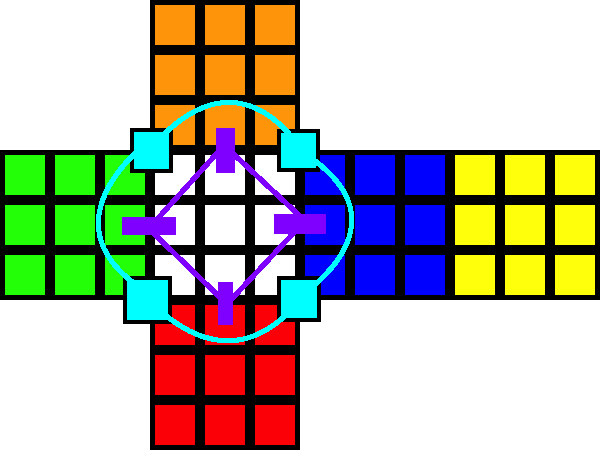
\includegraphics[scale=.5]{images/faceCubieCycle.png} 
\end{center}

We are only concerning ourselves with cycles of the cubies; stickers and orientations will be considered later.  It is clear that this face turn consists of two four-cycles: one of the edge cubies (purple) and one on the corner cubies (cyan).  Since these are cycles of even length, they are odd permutations in the symmetric subgroups concerning the respective cubie permutations.  This means that applying one face turn to the solved cube will bring the cubie permutations out of their respective alternating subgroups, and a second face turn would bring them back.  Thus, any face turn toggles the parity (sign) of \textit{both} symmetric subgroups in tandem.  This means that the symmetric edge and corner components $S_{\text{edges}}, S_{\text{corners}}$ satisfy
\begin{align*}
(S_{\text{edges}},S_{\text{corners}})
&\in
(\mathfrak{A}_{12} \times \mathfrak{A}_7)
\cup
(\bar{\mathfrak{A}_{12}} \times \bar{\mathfrak{A}_7})
\end{align*}
where $\mathfrak{A}_n$ is the alternating group of order n.  This is just a restatement of the fact that these parities in the symmetric subgroups must be equal. \\

This means that in a cube state in $O_s$, the edge positions are in an even parity with regards to their symmetric component if and only if the corners are as well, and likewise for odd parities.  Now, consider what happens if we apply a transposition on any two of the edges or corners.  WLOG, assume edges.  That will toggle the edge permutation parity, while preserving the parity of the corner pieces.  There is no legal move to fix this parity error, thus it is a different orbit.  This gives us a factor of 2 in the index $[\mathcal{A}_n : \mathcal{R}_n]$.

\subsection{Flipping An Edge}

In the first example of an illegal move, we focused on swapping two cubies without concern for any notion of ``orientation''.  We were merely concerned with the positions of the pieces, not their alignment.  This is enough to obtain a factor of 2 in the group index, or in other words, that the size of the Rubik Group $\mathcal{R}_n$ is at most half that of the size of the assembly group $\mathcal{A}_n$.  To continue with this question, however, we do need to talk about orientation of the cubies. \\

Orientation of the edge cubies is simpler than that of the corners, so we will start there.  Orientation can be arbitrarily chosen, and our choice of orientation systems will not affect the eventual result, however it will be easier to talk about orientation if we choose an intuitive definition.  We will choose an orientation scheme that is homogenous across all of the faces of the cube.  On each of the 12 edge cubies, we will choose one sticker and place a dot on it.  This can be done in such a way that every cube face has two dots on it, and in particular it will be nice if those dots are on opposite sides of the faces.  Then, we will also put dots on the center cubies adjacent to the edge dots.  This will be used later to determine what we mean by orientation.  Here is one such example.

\begin{center}
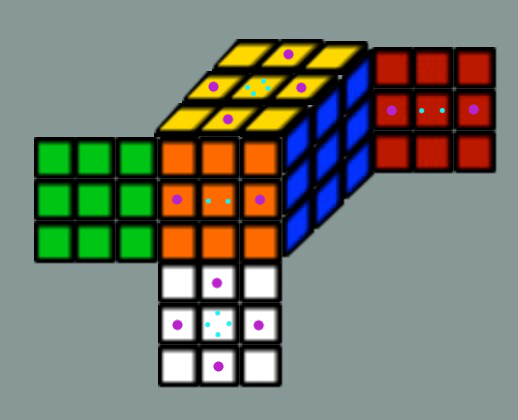
\includegraphics[scale=.65]{images/edgeOrientation.png} 
\end{center}

One important caveat of this physical representation is that the purple dots on the center stickers do not rotate with the underlying cubie.  While hardly realistic, this is important because if it weren't the case, then you could end up with two purple dots adjacent to different stickers of the same edge cubie, rendering our orientation scheme meaningless.  The purple dots are purely there for reference.  With this orientation in mind, though, we can construct a graph of the 24 possible edge position-orientation pairs and the transitions they can undergo with a legal move.  This number arises because there are 12 edges and any of them can be in one of two orientations.  We will call the orientations where the cyan dot is aligned with a purple dot ``positive'' and the other scenario ``negative'' orientation.  There are twelve of each, and it turns out that graphing them out results in a very nice bipartite graph such as this one.

\begin{center}
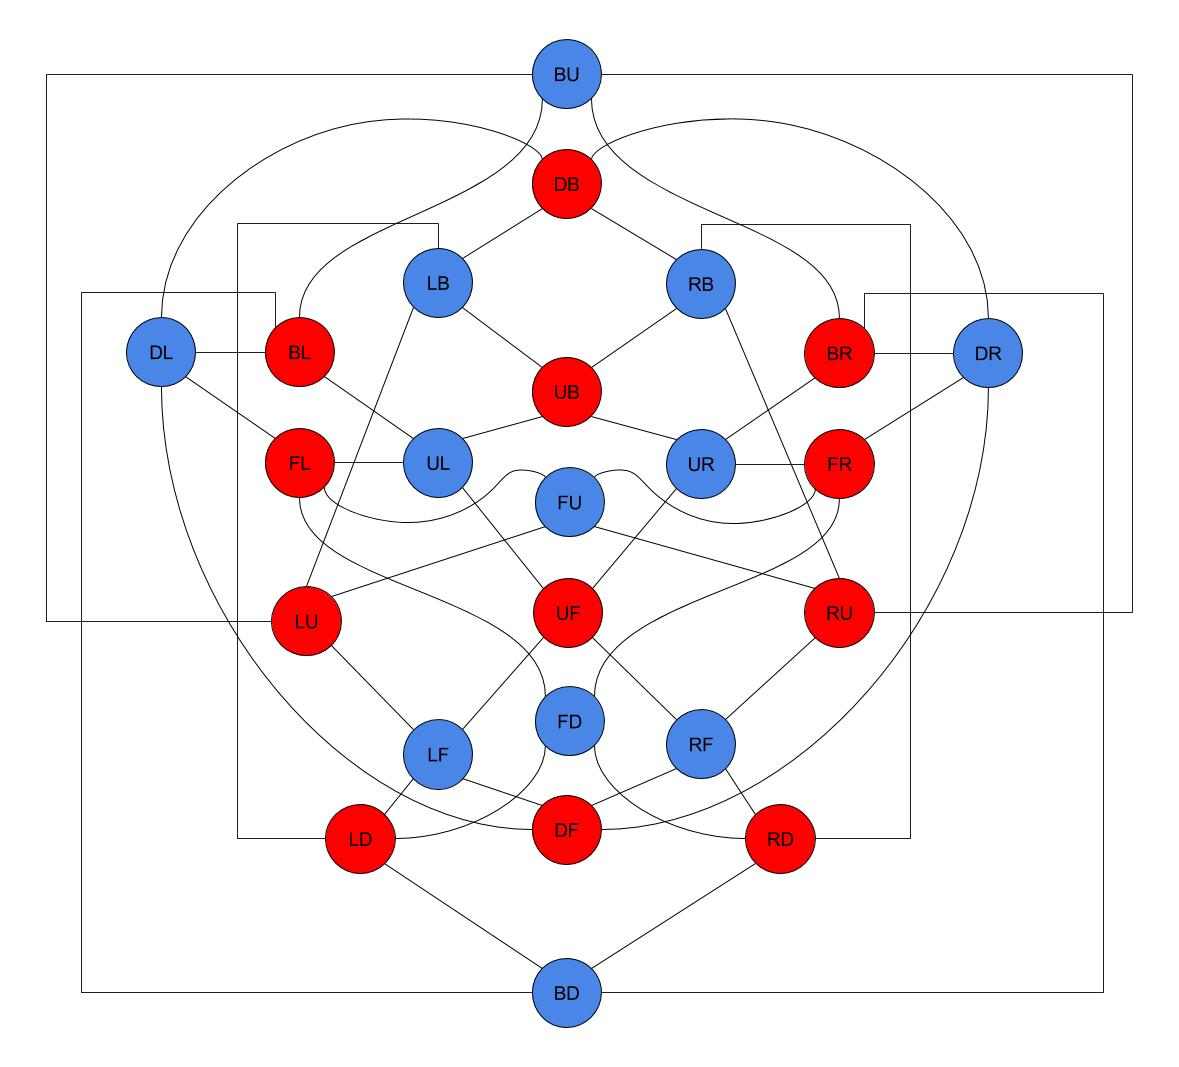
\includegraphics[scale=.35]{images/Rubiks_Edge_Graph.jpg} 
\end{center}

The bipartiteness of this graph is very significant.  It tells us that given an edge cubie in some arbitrary position and orientation, any turn of a face that contains it will flip it to the opposite orientation.  Because this is true of all four edge cubies involved in that Rubik's move, this tells us that we can never toggle the orientation of an odd number of edges with any legal moves.  This means that any reassembly of the cubies that contains an odd number of positively (or, equivalently, negatively) oriented edges in this scheme cannot be solved using legal moves.  This gives us a factor of at least 2 in our index of the Rubik's Group. \\

It is not immediately obvious, however, whether we can toggle the orientation of exactly two edges.  If this is impossible, then we have actually gained a factor of 4 rather than 2 in the index, as the number of positively-oriented edges for any legal state of the cube would have to be 0 mod 4 (i.e. one quarter of the possible assemblies).  The easiest way to disprove this possibility is to find a sequence of moves that flips in-place exactly two edges.  One such sequence is

\begin{align*}
(Ur)^4(U'r)^4
\end{align*}

Where the exponent signifies repetition of the steps and the lowercase r is, again, a slice move parallel to the right face. This sequence of moves flips in-place the UR and UL edges.  Using this knowledge, one can easily flip in-place any two arbitrary edges.  Simply conjugate the above sequence with a series of moves $S$ that puts the target edges into the UR and UL positions.  Moving the edge pieces there, flipping them, and then undoing the ``set-up moves'' as they are known to Rubik's Cube solvers is a safe, non-destructive way to flip any two arbitrary edges.  This knowledge combined with our previous statement from the graph proves that any cube state in the solvable orbit \textit{must} have an even number of positively-oriented edge pieces.  In particular, this shows that we gain a factor of exactly 2 in our index of the group, as desired.

\subsection{Rotating a Lone Corner}

We now wish to prove a similar result about the corner cubies.  While we could construct a graph similar to the one above for this purpose, it would not be as immediately useful.  The usefulness of the above graph came about primarily from its bipartiteness; a property that we were able to exploit.  Unfortunately, it is less clear what sort of ``graph property'' we could exploit for the corners, because they have three orientations rather than two.  Tripartiteness seems likely, but there is much less that we could say about a tripartite graph than a bipartite one.  Thus, we need to go a different route. \\

We still would like to find some sort of ``invariant'' about the solvable orbit that leads us to information about the orientation of the corners.  Towards that end, we will first assign an orientation to each corner cubie.  Note that every corner cubie has either a white sticker or a yellow sticker, as these are opposite faces on the cube.  We can use this to fix an orientation on each piece.  To each sticker on the corner cubies, we will assign a number in $\mathbb{Z}_3$.  The white and yellow stickers will be given zeroes, and we will write 1 and 2 on the other stickers in a clockwise fashion.  This results in the following labelling of the stickers.

\begin{center}
\includegraphics[scale=1.5]{images/cornerOrientation.png} 
\end{center}

We will now look at the sum of the numbers on the white and yellow faces (as determined by their colored centers).  We will show that applying any sequence of moves to the cube will always leave this sum unchanged.  Since the solved cube has an orientation sum of 0, this will show that all solvable cube assemblies \textit{must} have an orientation sum of 0. \\

We will look at each of the six standard face turns of the cube: U,D,L,R,F,B.  Assume without loss of generality that the white face is oriented up, and the red face is oriented to the front (as in the above picture).  Turning the white or yellow faces (U and D) are trivial with respect to corner orientation, as the numbers written on these faces will not change. \\

For the other four standard moves, we can observe that they are all isomorphic with respect to corner orientation.  Looking at the front face (red above), starting from the upper-left corner sticker and running clockwise around that face, we read off the sequence 1,2,1,2.  This is the same for any of the F,R,B,L faces.  Thus, we only need to test one of these turns and the result will be valid for any of the four.  Without loss of generality, we choose the red front face to rotate clockwise.  Doing so will result in the following cube configuration:

\begin{center}
\includegraphics[scale=1.5]{images/rotatedCornerOrientation.png} 
\end{center}

Adding up the numbers on the white and yellow faces again, they sum to $6 \cong_3 0$.  In particular, we need to look at what happened to each of the four corner cubies that have moved.  This table outlines where each cubie was (including orientation), where it went to, and the change in its orientation value.

\begin{center}
\begin{tabular}{|c|c|c|}
\hline 
From	 & To & Orientation Change mod 3 \\ 
\hline 
FUL (0) & FUR (2) & +1 \\ 
\hline 
FUR (0) & FDR (2) & -1 $\cong$ +2 \\ 
\hline 
FDR (0) & FDL (1) & +1 \\ 
\hline 
FDL (0 & FUL (2) & -1 $\cong$ +2 \\ 
\hline 
\end{tabular} 
\end{center}

Consider applying this move to an arbitrarily-assembled cube.  We don't know what the initial and final orientation values on these four cubies would be, but we do know that the orientation \textit{change} for each cubie will be the same as above.  This is guaranteed because of how we have defined the orientation scheme.  As stated above, this same sort of result would be obtained for turning any of the four faces that are neither the top nor bottom, and they have an even simpler case.  Thus, we have shown that no standard Rubik's move will change the orientation sum of its configuration, and because the solved state has orientation sum zero, so must all the solvable configurations. \\

Because exactly one third of possible assemblies have a corner orientation sum of zero, we have guaranteed that we will get at least a factor of 3 in the Rubik's Group index from this setup.  However, we have not yet shown that \textit{all} corner assemblies with orientation sum zero are solvable (which would make it exactly 3).  From what we have shown thus far, it could be the case that the solvable orbit of the cube does not contain every zero-orientation-sum assembly of the corners.  We will prove now that it, in fact, does. \\

We have shown from above that one cannot construct a sequence of valid moves to rotate in-place a single corner, leaving the orientations of the others fixed.  Doing so would alter the orientation sum, which cannot happen.  It is possible, however, to rotate two adjacent corners in tandem, one clockwise and the other anti-clockwise.  That is best shown by an example move sequence. \\

Let $S$ be the move sequence $R'D'RD$.  This is a standard one-line commutator in solving, and is a building block of the sequence we desire.  The entire sequence then looks like
\begin{align*}
S^2 U S^4 U' &= (R'D'RD)^2 U (R'D'RD)^4 U'
\end{align*}

This sequence rotates in-place the FUR and BUR corner cubies, the former being rotated counter-clockwise and the latter clockwise.  The resulting cube then looks like

\begin{center}
\includegraphics[scale=1.5]{images/twoCornersRotated.png} 
\end{center}

The orientation sum is still zero (as expected), as the orientation changes of these two counteract each other.  Note that this sequence can be easily adapted to rotate any two adjacent corners in a similar manner.  In fact, it can be adapted to rotate \textit{any} two corners similarly, but for our purposes we only need to know that any adjacent corners can be likewise rotated. \\

The easiest way to see this is to let the above sequence be denoted as $\hat{S}$, and then conjugate it by some sequence of moves that put the target two cubies in the FUR and BUR positions.  If this sequence consists of simple whole-cube turns, then we will be rotating adjacent corners, and more complex sequences can be used to rotate arbitrary corner-pairs.  Let $A$ be the sequence that moves the target two corners into the appropriate locations.  Then the sequence $A\hat{S}A^{-1}$ will perform the desired function.  It positions the target cubies appropriately, rotates them, and then moves them back to where they were.  This is totally non-destructive, as the only cubies affected by $\hat{S}$ are the corners being rotated. \\

With this knowledge in mind, we can now construct a simple vector space and use some linear algebra to prove our claim.  Let $V$ be the vector space over the field $\mathbb{Z}_3^8$ obtained by mapping an ordered-sequence of the 8 corner cubies to their localized orientations in a given \textit{solvable} cube configuration.   Let $W$ be the vector space over the same field such that the sum of the components is 0.  Our previous proof shows that $V$ is a subspace of $W$, but we do not yet know if it is a proper subspace. \\

Because we have shown that we can rotate any two adjacent corners in opposite directions, this gives rise to 12 generators for $V$.  These generators are column vectors $v$ such that $v_i = 1, v_j = 2 \Leftrightarrow $ corner cubies $i,j$ are adjacent.  We know that $W$ has dimension 7, as any vector can be thought of as 7 arbitrarily-chosen components, and then the eighth is fixed by the vector space description.  Thus, $V$ has dimension at most 7.  Assume for our purposes that we have ordered the 8 corner cubies as follows:

\begin{center}
\includegraphics[scale=1]{images/labelledWireframe.png} 
\end{center}

Then, we can look at seven such generating vectors that are the columns of the matrix

\begin{align*}
\begin{matrix}
1 & 0 & 0 & 0 & 0 & 0 & 0 \\ 
2 & 1 & 0 & 0 & 0 & 0 & 0 \\ 
0 & 2 & 1 & 0 & 0 & 0 & 0 \\ 
0 & 0 & 2 & 1 & 0 & 0 & 0 \\ 
0 & 0 & 0 & 2 & 1 & 0 & 0 \\ 
0 & 0 & 0 & 0 & 2 & 1 & 0 \\ 
0 & 0 & 0 & 0 & 0 & 2 & 1 \\
0 & 0 & 0 & 0 & 0 & 0 & 2 
\end{matrix} 
\end{align*}

The columns of this matrix are independent, meaning its rows are 7 independent vectors in $W$.  Because all of these vectors can be realized in $V$ as well, and the number of vectors is equal to the dimension of $W$, we know that $V=W$.  This tells us that a cube assembly with a corner orientation sum of zero, corners can be rotated such that they are solved using legal moves.  This tells us that we obtain a factor of exactly 3 in the index of the Rubik's Group from the corner orientations.

\subsection{Cardinality of the Group}
From what we have proven in the previous few sections, we know that the index of the Rubik-3 Group in the Assembly-3 group, written $[\mathcal{R}_3 : \mathcal{A}_3] = 30 \cdot 2 \cdot 2 \cdot 3 = 360$.  Thus, the size of the Rubik Group can be calculated as \begin{align*}
|\mathcal{R}_3| &= \frac{|\mathcal{A}_3|}{30 \cdot 2 \cdot 2 \cdot 3} \\
&= \frac{7! \cdot 3^7 \cdot 12! \cdot 2^{12} \cdot 6!}{30 \cdot 2 \cdot 2 \cdot 3} \\
&\approx 4.3252003 \times 10^{19}
\end{align*}

There is an important note to make here about how we handled duplicate ``assemblies'' in the assembly group.  To account for this, we fixed one corner piece in both position and orientation.  It is not immediately obvious how this was handled in the Rubik's Group or its index, but this was actually not a concern.  Because we never included any whole-cube rotations in $\mathcal{R}_3$, there is no way for duplicates to arise.  In this group, the center pieces are fixed and handle orientation of the puzzle, preventing duplicates.  To map this to an element of $\mathcal{A}_3$, one simply needs to locate the ``fixed'' corner cubie, and turn the cube as a whole to properly position and orient this cubie as needed for the assembly group. \\

While this distinction could be important in describing the intricacies of $\mathcal{R}_3$ as a subgroup of $\mathcal{A}_3$, it is not important in talking about cardinalities.  To be pedantic, one could describe a group isomorphic to $\mathcal{R}_3$ that rotates cube states appropriately, and \textit{that} group would technically be a subgroup of $\mathcal{A}_3$.  If this distinction becomes important at a latter point, we will address it then.  For now, it is best left down in the weeds.
\end{document}